%%%%%%%%%%%%%%%%%%%%%%%%%%%%%%%%%%%%%%%%%
% Structured General Purpose Assignment
% LaTeX Template
%
% This template has been downloaded from:
% http://www.latextemplates.com
%
% Original author:
% Ted Pavlic (http://www.tedpavlic.com)
%
% Note:
% The \lipsum[#] commands throughout this template generate dummy text
% to fill the template out. These commands should all be removed when 
% writing assignment content.
%
%%%%%%%%%%%%%%%%%%%%%%%%%%%%%%%%%%%%%%%%%

%----------------------------------------------------------------------------------------
%	PACKAGES AND OTHER DOCUMENT CONFIGURATIONS
%----------------------------------------------------------------------------------------

\documentclass{article}

\usepackage{fancyhdr} % Required for custom headers
\usepackage{lastpage} % Required to determine the last page for the footer
\usepackage{extramarks} % Required for headers and footers
\usepackage{graphicx} % Required to insert images
\usepackage{lipsum} % Used for inserting dummy 'Lorem ipsum' text into the template
\usepackage{listings}
\usepackage{color}
\usepackage{amsmath}

\definecolor{dkgreen}{rgb}{0,0.6,0}
\definecolor{gray}{rgb}{0.5,0.5,0.5}
\definecolor{mauve}{rgb}{0.58,0,0.82}

\lstset{frame=tb,
  language=c,
  aboveskip=3mm,
  belowskip=3mm,
  showstringspaces=false,
  columns=flexible,
  basicstyle={\small\ttfamily},
  numbers=none,
  numberstyle=\tiny\color{gray},
  keywordstyle=\color{blue},
  commentstyle=\color{dkgreen},
  stringstyle=\color{mauve},
  breaklines=true,
  breakatwhitespace=true
  tabsize=3
}

% Margins
\topmargin=-0.45in
\evensidemargin=0in
\oddsidemargin=0in
\textwidth=6.5in
\textheight=9.0in
\headsep=0.25in 

\linespread{1.1} % Line spacing

% Set up the header and footer
\pagestyle{fancy}
\lhead{\hmwkAuthorName} % Top left header
\chead{\hmwkClass\ (\hmwkClassInstructor\ \hmwkClassTime): \hmwkTitle} % Top center header
\rhead{\firstxmark} % Top right header
\lfoot{\lastxmark} % Bottom left footer
\cfoot{} % Bottom center footer
\rfoot{Page\ \thepage\ of\ \pageref{LastPage}} % Bottom right footer
\renewcommand\headrulewidth{0.4pt} % Size of the header rule
\renewcommand\footrulewidth{0.4pt} % Size of the footer rule

\setlength\parindent{0pt} % Removes all indentation from paragraphs

%----------------------------------------------------------------------------------------
%	DOCUMENT STRUCTURE COMMANDS
%	Skip this unless you know what you're doing
%----------------------------------------------------------------------------------------

% Header and footer for when a page split occurs within a problem environment
\newcommand{\enterProblemHeader}[1]{
\nobreak\extramarks{#1}{#1 continued on next page\ldots}\nobreak
\nobreak\extramarks{#1 (continued)}{#1 continued on next page\ldots}\nobreak
}

% Header and footer for when a page split occurs between problem environments
\newcommand{\exitProblemHeader}[1]{
\nobreak\extramarks{#1 (continued)}{#1 continued on next page\ldots}\nobreak
\nobreak\extramarks{#1}{}\nobreak
}

\setcounter{secnumdepth}{0} % Removes default section numbers
\newcounter{homeworkProblemCounter} % Creates a counter to keep track of the number of problems

\newcommand{\homeworkProblemName}{}
\newenvironment{homeworkProblem}[1][Problem \arabic{homeworkProblemCounter}]{ % Makes a new environment called homeworkProblem which takes 1 argument (custom name) but the default is "Problem #"
\stepcounter{homeworkProblemCounter} % Increase counter for number of problems
\renewcommand{\homeworkProblemName}{#1} % Assign \homeworkProblemName the name of the problem
\section{\homeworkProblemName} % Make a section in the document with the custom problem count
\enterProblemHeader{\homeworkProblemName} % Header and footer within the environment
}{
\exitProblemHeader{\homeworkProblemName} % Header and footer after the environment
}

\newcommand{\problemAnswer}[1]{ % Defines the problem answer command with the content as the only argument
\noindent\framebox[\columnwidth][c]{\begin{minipage}{0.98\columnwidth}#1\end{minipage}} % Makes the box around the problem answer and puts the content inside
}

\newcommand{\homeworkSectionName}{}
\newenvironment{homeworkSection}[1]{ % New environment for sections within homework problems, takes 1 argument - the name of the section
\renewcommand{\homeworkSectionName}{#1} % Assign \homeworkSectionName to the name of the section from the environment argument
\subsection{\homeworkSectionName} % Make a subsection with the custom name of the subsection
\enterProblemHeader{\homeworkProblemName\ [\homeworkSectionName]} % Header and footer within the environment
}{
\enterProblemHeader{\homeworkProblemName} % Header and footer after the environment
}
   
%----------------------------------------------------------------------------------------
%	NAME AND CLASS SECTION
%----------------------------------------------------------------------------------------

\newcommand{\hmwkTitle}{Assignment\ \#5} % Assignment title
\newcommand{\hmwkDueDate}{Monday,\ Mar 24,\ 2014} % Due date
\newcommand{\hmwkClass}{Computational Biology} % Course/class
\newcommand{\hmwkClassTime}{1:30pm} % Class/lecture time
\newcommand{\hmwkClassInstructor}{Jianyang Zeng} % Teacher/lecturer
\newcommand{\hmwkAuthorName}{Weiyi Chen} % Your name

%----------------------------------------------------------------------------------------
%	TITLE PAGE
%----------------------------------------------------------------------------------------

\title{
\vspace{2in}
\textmd{\textbf{\hmwkClass:\ \hmwkTitle}}\\
\normalsize\vspace{0.1in}\small{Due\ on\ \hmwkDueDate}\\
\vspace{0.1in}\large{\textit{\hmwkClassInstructor\ \hmwkClassTime}}
\vspace{3in}
}

\author{\textbf{\hmwkAuthorName}}
\date{} % Insert date here if you want it to appear below your name

%----------------------------------------------------------------------------------------

\begin{document}

\maketitle

%----------------------------------------------------------------------------------------
%	TABLE OF CONTENTS
%----------------------------------------------------------------------------------------

%\setcounter{tocdepth}{1} % Uncomment this line if you don't want subsections listed in the ToC

%\newpage
%\tableofcontents
\newpage

%----------------------------------------------------------------------------------------
%	PROBLEM 1
%----------------------------------------------------------------------------------------

% To have just one problem per page, simply put a \clearpage after each problem

\begin{homeworkProblem}
	Dead End Elimination (DEE) Pruning
	\begin{homeworkSection}{(1) Prove the theorem}
		\centerline{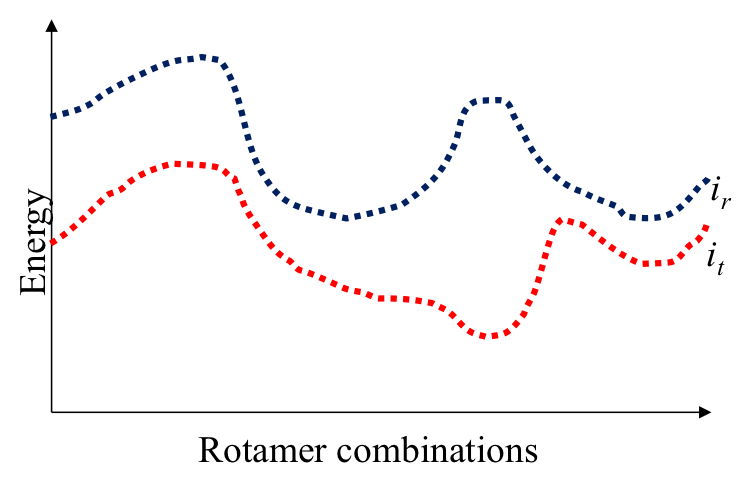
\includegraphics[scale = 0.5]{dde2.png}}
		Assume by contradiction that rotamer $i_r$ is part of optimal solution in some case, namely there exist some combination of $j$ such that
		$$ \sum_j [E(i_r, j_s) - E(i_t, j_s)] < 0 $$
		This implies that 
		$$ \text{min}_s \sum_j [E(i_r, j_s) - E(i_t, j_s)] < 0 $$
		However, it is easy to figure out 
		$$ \text{min}_s \sum_j [E(i_r, j_s) - E(i_t, j_s)] \ge \sum_j \text{min}_s [E(i_r, j_s) - E(i_t, j_s)] $$ 
		This is because in the left part, the combination of $j$ is defined before deriving minimal, which is possibly to exist. But in the right part of the inequality, it is deriving the minimal of each $j_s$ before summing up. So there're some cases, like different $j_s$ in each element of the sum is not possible to exist at the same time. In other words, cases in the right part cover the left part, so it's able to get a smaller value. \\
		Since  
		$$ \sum_j \text{min}_s [E(i_r, j_s) - E(i_t, j_s)] > 0 $$
		We have
		$$ \text{min}_s \sum_j [E(i_r, j_s) - E(i_t, j_s)] > 0 $$
		which contradicts to our assumption.
	\end{homeworkSection}
	\begin{homeworkSection}{(2) Analyze the time complexity}
		Let $N$ be the number of amino acid positions, as above, and let $p$ be the number of rotamers at each position (this is usually, but not necessarily, constant over all positions). Given this model, it is clear that the DEE algorithm is guaranteed to find the optimal solution; that is, it is a global optimization process. The single-rotamer search scales quadratically in time with total number of rotamers. The pair search scales cubically and is the slowest part of the algorithm (aside from energy calculations). This is a dramatic improvement over the brute-force enumeration which scales as $O(p^{N})$.
	\end{homeworkSection}
\end{homeworkProblem}

%----------------------------------------------------------------------------------------
%	PROBLEM 2
%----------------------------------------------------------------------------------------

% To have just one problem per page, simply put a \clearpage after each problem

\begin{homeworkProblem}
	A* Search
	\begin{homeworkSection}{(1) Prove the theorem}
		If the heuristic function h is admissible, meaning that it never overestimates the actual minimal cost of reaching the goal, then A* is itself admissible (or optimal) if we do not use a closed set. If a closed set is used, then h must also be monotonic (or consistent) for A* to be optimal. This is to prove, problems with a consistent heuristics cannot be solved any better than A* can solve them by algorithms with the same information.\\
		Defined by a quadruple: $I = (G, s, \Gamma, h)$, where
		\begin{itemize}
			\item $G$ is the graph representation of the problem
			\item s is the start node in the graph
			\item $\Gamma$ is the set of goal nodes
			\item h is a heuristic that any algorithm run on this instance will use
		\end{itemize}
		Given a set of problem instance $I = (G, S, \Gamma, h) $, and assuming n is surely expanded by A*, then there exists a path $P_{s-n}$ s.t.
		$$ \forall n' \in P_{s-n}, g(n') + h(n') < C* $$
		where 
		\begin{itemize}
			\item $P_{n_i - n_j}$ is a path in G between the node $n_i$ and $n_j$
			\item $g(n)$ is the sum of the branch costs along the current path of pointers from n to s
			\item $f(.)$ is the evaluation function de?ned over partial paths, i.e., to  to each node n
along a given path $P = s_1, n_1, n_2, ..., n$ we assign the value $f_P(n)$ which is shorthand notation for $f(s, n_1, n_2, ..., n)$
			\item C* is the cost of the cheapest solution path 
		\end{itemize}
		Let B be an algorithm compatible with A* that halts with cost C* in I. Assume that B does not expand n. We can then create G'. What we do here is setup a contradiction: For B to be better than A*, it must skip some node n that A* visits. We assume B does this, and setup a new graph G' that will introduce a contradiction.
		\centerline{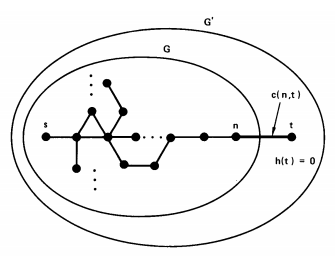
\includegraphics[scale = 0.5]{astar}}
		where we have added a goal node t to G. The costs of t is given by $h(t) = 0$ and the edge from n to t is given as $c = h(n) + \Delta$ where:
		$$ \Delta = \frac{1}{2} (C^* - D) > 0 $$
		$$ D = \text{max} \{ f(n') | n' \in N_{g+h}^{G^*} \} $$
		This creates a new path P* whose cost is $\le C^* - \Delta$ yet is still consistent (and admissible) on the new I'. Here, we setup a new node in G0 and make sure it has the proper costs associated with it so that the new G' obeys all the rules that the old G did. \\
		It remains to be proven that h is consistent on I' for the new node t in G' (this is trivially true for all the previous nodes since the h values of all the nodes in G remain unchanged). This is done by establishing $h(n') \le k(n', t) \forall n' \in G $. At any node n' we should also have
		$$ h(n') > k(n', n) + c = k(n', n) + h(n) + \Delta $$
		We show that by using the above weight for the $k(n', t)$ edge, the new graph G' remains consistent.
		Thus A* will ?nd the new path P* (which costs $C^* - \Delta$) because
		$$ f(t) = g(n) + c = f(n) + \Delta = D + \Delta = C^* - \Delta < C^* $$
		So t is reachable from s by a $C^* - \Delta$ bounded path, so it will be selected. \\
		But algorithm B must behave the same as if it were running on I, halting with cost $C^* > C^* - \Delta$  This is a contradiction that B is both admissible on I, and avoids the expansion of n. \\
		We have a contradiction, because after creating G', which has a shortest path goal node attached to n (which A* finds properly), B is unable to find a shortest path and therefore must not be admissible.
	\end{homeworkSection}
	\begin{homeworkSection}{(2) What is the relationship between Dijkstra and A* search algorithms?}
		The A* algorithm is a generalization of Dijkstra's algorithm that cuts down on the size of the subgraph that must be explored, if additional information is available that provides a lower bound on the "distance" to the target. This approach can be viewed from the perspective of linear programming: there is a natural linear program for computing shortest paths, and solutions to its dual linear program are feasible if and only if they form a consistent heuristic (speaking roughly, since the sign conventions differ from place to place in the literature). This consistent heuristic defines a non-negative reduced cost and A* is essentially running Dijkstra's algorithm with these reduced costs.
	\end{homeworkSection}
\end{homeworkProblem}

\end{document}